\chapter{Introduction}

\section{Motivation}


Taking long term decisions or spontaneous reactive actions when presented with incomplete information or partial knowledge is 
paramount to the survival of any biological or synthetic entity. Reasoning given a state of uncertainty is a continuously occurring event throughout our 
livelihood. When considering long term decisions an abundance of examples come to mind. For instance, in economic investments 
uncertainty is to the best of efforts quantified and minimised in order to avoid unwarranted risks. Reactive actions are just as common; 
when looking for the snooze button of an alarm clock, early in the morning, our hand seems to autonomously search the surrounding space picking up
sensory cues gradually acquiring information guiding us towards the button. All the above types of decision require the integration of 
evidence and an ability to predict the outcomes of the taken decisions in order to insure a favourable end state. 
The ability to reason, in Artificial Intelligence (AI) \& robotics, whilst taking uncertainty into consideration has 
resulted in mixed levels of success. 

% Solving decision problem for structured problems [Operational Research]; backgammon, chess or go, where the adversiary can be considered
% a source of uncertainty.

There has been noticeable success in artificial agents beating humans at board games such as backgammon 
(TD-Backgammon), chess (Deep blue) and now recently go (AlphaGo). The gap between robotic autonomous systems and humans  starts to diverge when the action space is continuous and 
uncertainty is non-negligible. Although there are recent example of robots coping with such conditions: opening doors (pose and shape uncertainty of the handle),
walking down stairs (state transition uncertainty)(Asimo), and turning valves (DARPA Robotic challenge, DAC \cite{DARPA_2015}), repetition and reproducibility of such behaviour 
is hard. This was highlighted in the results of the 2015 DAC in which issues (perception, control, etc...) resulted in many robots
loosing balance and falling \footnote{\url{http://www.cs.cmu.edu/~cga/drc/}}. There is increasing amount of robotic application domains in which 
perception is limited, such as planetary\footnote{\url{http://exploration.esa.int/mars/}} and deep water exploration, in which 
optimal decisions under uncertainty play a critical role in the success of the tasks undertaken. It would be advantageous to leverage
human decision and action abilities for tasks in which the effect of uncertainty is problematic, such as exploration, search and manipulation.

\begin{figure}
 \centering
 \includegraphics[width=\textwidth]{examples2.pdf}
 \caption{Examples of the decision making under uncertainty in both robotics and everyday life situations. (a) European Space Agency (ESA), remote orbital peg in hole task. (b)-(c) 
 ESA, simulated exploration of a cave on Mars in the dark. (d)-(e) MIT DAC team, Atlas robot doing valve task, \url{http://drc.mit.edu/}. Other pictures include underwater 
 exploration and industrial peg-in-hole assembly.}
\end{figure}

It is not yet fully understood how decisions are taken, yet alone under uncertainty. The difficulty is that two processes responsible 
for the synthesis of our actions and decisions, our beliefs and desires, are not directly or easily measurable. There is growing interest in 
Neuroscience to understand the mechanisms underlying perception and decision making under uncertainty, \cite{decision_un_2013}; there is not 
yet a consensus on the biological mechanisms involved in decision making and efforts are 
ongoing\footnote{the human brain project: https://www.humanbrainproject.eu/} to construct plausible models of our decision processes. 

%At a behavioural level, early efforts to model human decision making were made in mathematics \& economics 
%(\cite{Bernoulli1954},\cite{VonNeumann1944}), in which gambles and investments were chiefly considered. There has been 
%considerable effort in many fields (neuroscience, cognitive science, physiology, economics, etc..) to understand how decisions and actions 
%are taken, starting with the role of our neurons to high level decisions like gambling, orientation and navigation problems to reflexes. 
% 3) Aritficiel intelligence & robots (How is uncertainty taken into account in the decision process)


AI \& robotics considered early on uncertainty in decision making, 
where the predominant domain of application was spatial navigation, \cite{ActingUncertainty_1996}. The problem has 
always been treated in two parts: the construction and representation of a world model (the map) and a planner which can reason with 
respect to this model in order to accomplish an objective. The world construction problem attracted a large amount of 
interest and has resulted in many successfully applications in a wide spectrum of robotic domains (AUV, UAV, etc..). 

The integration of planning with mapping in a single framework is still difficult to achieve and is based on either 
representing the decision problem as a Partially Observable Markov Decision Process (POMDP) which is notoriously difficult 
to solve for large scale problems or by search heuristics.  



%The mapping problem can generally be solved when assuming the uncertainty is Gaussian and thus quantifiable by a few parameters.
%The current frontier in planning and reasoning under uncertainty includes both discrete and continuous problems in which the uncertainty
%is constrained to a few state variables or is Gaussian. 

In summary there are still open problems in decision making when considering partial observability.
As both humans and animals are far better at navigation than robots, especially when uncertainty is present, \cite{stankiewicz2006lost},
we decide to leverage human foresight and reasoning in a Programming by Demonstration (PbD) framework (\cite{Billard08chapter}). 
PbD examples include the transfer of kinematic task constraints, stiffness and impedance constraints and motion primitives, to name only a few.

The mapping problem has been studied and solved within a certain set of constraining assumptions. For the mapping problem we
develop a Bayesian filter which is non-parametric and has no explicit representation of a joint distribution.

In this thesis we address both mapping and planning problems under extreme levels of uncertainty. 


%The advantage of taking a LfD approach and encoding the demonstrated behaviour in a asynchronous dynamical system (ADS) is that we have robustness to perturbation
% and a generalisation over the entire state space. 

\section{Contribution}
% - One page 1/2 
%	PbD-POMDP 
%	Evaluation of the behaviour present in humans, Can humans be suitable teachers to show robots how to act 
%	when under extreme levels of uncertainty.
%	
%	RL-PbD-POMDP: Given a simple objective function we can use this to boostrap the apprentiship learning as a means
%		      to select actions which are better.
%
%	Large amount of uncertainty.

In this thesis we bring to light three contributions:

\begin{enumerate}
 \item[\ref{sub:contr1}] \hyperref[sub:contr1]{Learning to reason with uncertainty as humans.}\\
 The first is the transfer of human behaviour, through learning a parametric policy, to robots in tasks where 
 a lot of uncertainty in present, making them difficult to solve using traditional techniques.
 \item[\ref{sub:contr2}] \hyperref[sub:contr2]{Reinforcement learning in belief space.}\\
 The second is an extension of the first, we add cost function which we demonstrate can be used 
 to refine and improve an original policy solely learned from human demonstrations.
 \item[\ref{sub:contr3}] \hyperref[sub:contr3]{Non-parametric Bayesian state space filter.}\\
 The third is a non-parametric Bayesian state space filter which is efficient under sparse sensory information 
and high levels of uncertainty.

\end{enumerate}


Throughout the work in this thesis we consider case studies in which vision is not available, leaving tactile and 
haptic information. This choice was made to induce a high level of uncertainty making it easier to study its effect 
on the decision making process. As a consequence the tasks we consider are by nature, haptic and tactile searches.
The following three sections detail the contribution of this thesis to research decision making under sever 
uncertainty constraints.

\subsection{Learning to reason with uncertainty as humans}\label{sub:contr1}

A Markov Decision Process (MDP) allows the formulation of a decision problem in terms of states, actions, a discount factor 
and a cost function. Given this formulation and a suitable optimisation method (dynamic programming, temporal difference, etc..) 
a set of optimal decision rules are returned, known as a policy. The benefit of this approach 
is that the policy is non-myopic and sequences of complicated actions can be synthesised to achieve a goal which 
an opportunistic policy would fail to achieve. A Partially Observable Markov Decision Process (POMDP) is 
a generalisation of an MDP to a hidden state space and only observations are available relating 
to the state space. Finding an exact optimal solution to a POMDP problem is notoriously difficult due to 
the computational complexities involved. Sample based approaches to solve a POMDP rely heavily on 
a good trade-off between exploration and exploitation actions. Good explorative actions increase the chance of discovering 
a set of optimal decisions/actions.

In this thesis we propose a Programming from Demonstration approach to solving POMDP problems in
haptic and tactile search tasks. Our hypothesis is that if we know the mental state of the human 
expert in terms of his believed location and observe his actions we can learn a statistical policy 
which mimics his behaviour. Since the human's beliefs are not directly observable we infer them 
by assuming that the way we integrate evidence is similar to a Bayesian filter. There is   
evidence both in cognitive and neuroscience that this is the case (\cite{Bake_Saxe_Tene_2011}). From 
observing the expert human performing a task we learn a cognitive model of the human's decision process 
by learning a generative joint distribution over his beliefs and actions. The generative distribution 
is then used as a control policy. By this approach we are able to have a policy which can handle uncertainty
similarly to humans. 

\subsection{Reinforcement learning in belief space}\label{sub:contr2}

% Disconnected with the previous section. 
Learning to search and act as humans and reproduce the exploratory behaviour is beneficial in POMDP tasks since
it is infeasible to use traditional solvers. The drawback of this approach is that the goal of the task is 
implicitly encoded in the demonstrations of the teacher. As a result the quality of the learned behaviour 
will depend on the skill and embodiment constraints of the human. Reinforcement learning (RL) is a framework which 
allows, through repeated interaction with the environment, to learn an optimal policy for a task. There are 
many variants of RL, but all rely on simple exploration strategies to find the optimal behaviour. These explorative 
strategies prohibited the application of RL to large and continuous POMDP settings in which the policy 
comprises of many parameters. In our previous contribution we showed that it is feasible to learn and extract 
multiple search strategies from the human demonstrations and in a sense have already solved the exploration/exploitation dilemma which 
plagues reinforcement learning applications. 

We propose a Reinforcement Learning framework for the task of searching and connecting a power plug to a socket, 
with only haptic information. 
We previously addressed this setup by learning a generative model of the beliefs and actions with data 
provided by human demonstrations following the LfD approach. However, it is usually the requirement that 
the teacher is an expert, with few notable exceptions (\cite{rai2013learning}). Since we were solely learning a 
statistical controller, both good and bad demonstrations will be mixed in together. By introducing a cost function 
representing the task we can explicitly have a quality metric of the provided demonstrations. In this way 
we can optimise the parameters of our generative model to maximise the cost function. In this LfD Reinforcement 
Learning setup with a very simple cost function we can have a significant improvement of our a policy.

\subsection{Non-parametric Bayesian state space filter}\label{sub:contr3}

%	Need an introduction, no big jump.
%
%

Simultaneous Localisation and Mapping (SLAM) is concerned with the development of filters to accurately and efficiently infer 
the state parameters of an agent (position, orientation) and aspects of its environment, commonly referred to as the map. 
It is necessary for the agent to achieve situatedness which is a precondition to planning and reasoning. The 
predominant assumption in most applications of SLAM algorithms is that uncertainty is related to the noise in the sensor measurements. In 
our haptic search tasks there is no visual information and a very large amount of uncertainty. Most of the sensory
feedback is negative information, a term used to denote the non event of a sensory response.
In the absence of recurrent sightings or direct measurements of objects there are no correlations from the measurement errors 
which can be exploited. 

In this thesis we propose a new SLAM filter, which we name Measurement Likelihood Memory Filter (MLMF), in 
which no assumptions are made with respect to the shape of the uncertainty (it can be Gaussian, multi-modal, uniform, etc..) and 
motion noise. We adopt a histogram parametrisation (this is considered non-parametric because a change in a parameter has a local effect). 
The conceptual difference between the MLMF and standard SLAM filters, 
such as the Extended Kalman Filter (EKF), is that we avoid representing the joint distribution since it would entail a shattering space and time complexity. 
This is achieved by keeping track of the history of measurement likelihood functions. We demonstrate that our approach gives 
the same filtered marginals as a histogram filter. In such a way we achieve a Bayes filter which has both linear space and 
time complexity. This filter is well suited to tasks where the landmarks are not directly observable.


\begin{figure}
  \centering
  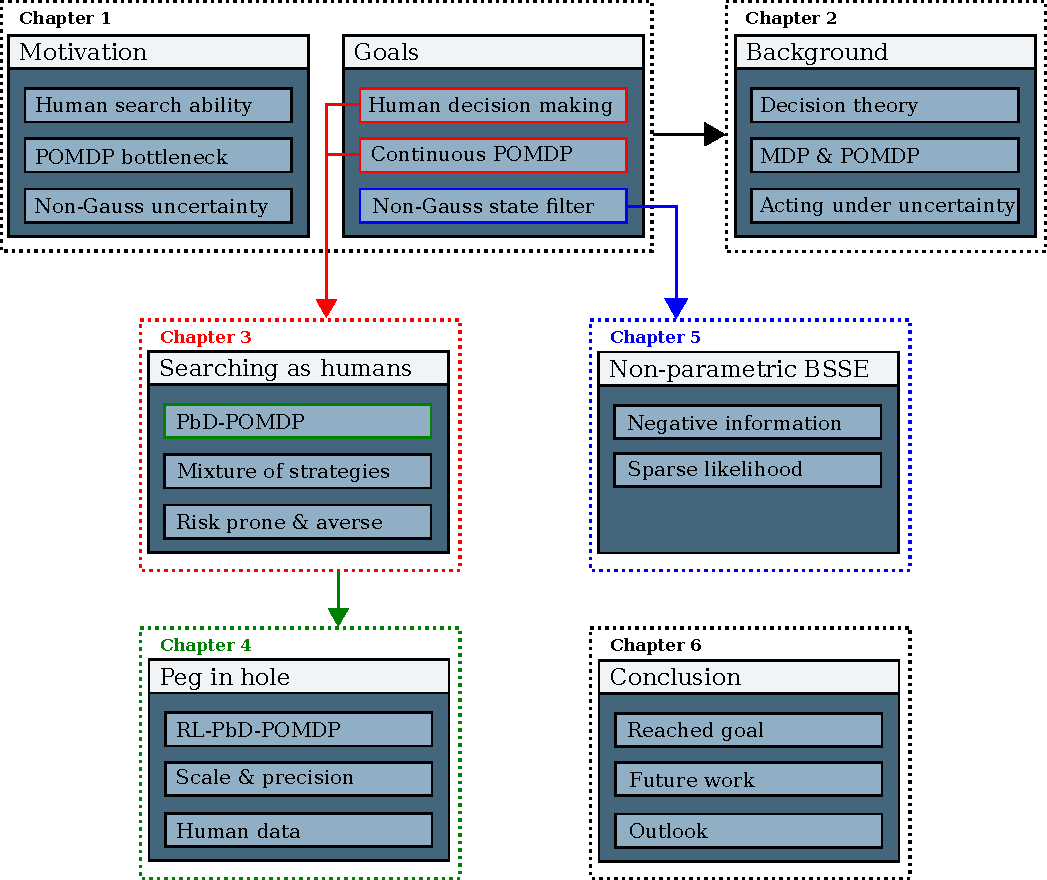
\includegraphics[width=\textwidth]{roadmap.pdf}
  \caption{Roadmap of the Thesis with key points. }
\end{figure}

\section{Thesis outline}

The thesis is structured accordingly to the three main contributions outlined in the previous section, 
and all will have their individual chapter. We outline below the structure of the thesis.

\begin{minipage}[c]{0.9\textwidth}
\paragraph{Chapter 2 - Background}\\
In this chapter we introduce and mathematically formalise the sequential decision making problem 
under uncertainty and we provide a detailed literature review of the related work in this domain.
We provide a brief introduction to \textit{Decision Theory} before focusing on the work 
in AI \& robotics relevant to POMDPs whilst highlighting their relevance and contribution to our work. 
\end{minipage}

\begin{minipage}[c]{0.9\textwidth}
\paragraph{Chapter 3 - Learning to reason with uncertainty as humans}\\
In this chapter we present an approach for transferring human skills in a blind haptic 
search task to a robot. The belief of the human is represented by a particle filter and 
all subsequent beliefs are inferred from the human's motions acquired via a motion tracking
system. A generative model of the joint belief and actions distribution is learned and used
to reproduce the behaviour on a WAM and KUKA robot in two search tasks. Experimental 
evaluations showed the approach to be superior to greedy opportunistic policies and traditional
path planning algorithms. 
We also provide a review of work related to humans taking decisions under uncertainty 
in spatial navigation and haptic tasks with an emphasis on works which consider diminished or no 
visual information. 
\end{minipage}

\begin{minipage}[c]{0.9\textwidth}
\paragraph{Chapter 4 - Reinforcement learning in belief space}\\
In this chapter we present an approach similar to the one presented in Chapter 3, ``Learning to reason with uncertainty as humans'', with the difference that
we explicitly encode the task through the introduction of a binary objective function and we consider a peg-in-hole
task under high levels of uncertainty. The task requires both high and low levels or precision to be able to accomplish it,
which makes it particularly interesting. We learn a value function approximation of the belief space through locally weighted 
regression and approximate dynamical programming.
By combining a LfD approach in this Actor-critic Reinforcement Learning framework, we demonstrate an improvement upon 
a purely statistical controller with nearly no additional cost. 
We additionally provide a review of RL methods in the context of POMDPs.
\end{minipage}

\begin{minipage}[c]{0.9\textwidth}
\paragraph{Chapter 5 - Non-parametric Bayesian state space filter}\\
In this chapter we present an approach to perform a state space estimation of a map and agent 
given that there is no direct observation between the landmarks and the agent. We demonstrate that 
by not explicitly parametrizing the full joint distribution of the landmarks and agent but instead
keeping track of the applied measurement functions we can fully reconstruct the optimal Bayesian 
state estimation. The advantage of our approach is that the space complexity is linear as oppose 
to exponential. We validate our approach in 2D search navigation tasks.
We also give an overview of the literature of SLAM and emphasis the position of our filter within it.
\end{minipage}

\begin{minipage}[c]{0.9\textwidth}
\paragraph{Chapter 6 - Conclusion}\\
We conclude by providing a holistic summary of our work and achievements. We draw attention to the current 
open problems and directions for future work in field of uncertainty and reasoning in Artificial intelligence and robotics.
\end{minipage}







